\documentclass[12pt]{article}

\usepackage{amssymb,amsmath,amsthm}
\usepackage[top=1in, bottom=1in, left=1.25in, right=1.25in]{geometry}
\usepackage{fancyhdr}
\usepackage{enumerate}
\usepackage[bw,framed,numbered]{mcode}
\usepackage{graphicx}

% Comment the following line to use TeX's default font of Computer Modern.
\usepackage{times,txfonts}

\newtheoremstyle{homework}% name of the style to be used
  {18pt}% measure of space to leave above the theorem. E.g.: 3pt
  {12pt}% measure of space to leave below the theorem. E.g.: 3pt
  {}% name of font to use in the body of the theorem
  {}% measure of space to indent
  {\bfseries}% name of head font
  {:}% punctuation between head and body
  {2ex}% space after theorem head; " " = normal interword space
  {}% Manually specify head
\theoremstyle{homework} 

% Set up an Exercise environment and a Solution label.
\newtheorem*{exercisecore}{Exercise \@currentlabel}
\newenvironment{exercise}[1]
{\def\@currentlabel{#1}\exercisecore}
{\endexercisecore}

\newcommand{\localhead}[1]{\par\smallskip\noindent\textbf{#1}\nobreak\\}%
\newcommand\solution{\localhead{Solution:}}

%%%%%%%%%%%%%%%%%%%%%%%%%%%%%%%%%%%%%%%%%%%%%%%%%%%%%%%%%%%%%%%%%%%%%%%%
%
% Stuff for getting the name/document date/title across the header
\makeatletter
\RequirePackage{fancyhdr}
\pagestyle{fancy}
\fancyfoot[C]{\ifnum \value{page} > 1\relax\thepage\fi}
\fancyhead[L]{\ifx\@doclabel\@empty\else\@doclabel\fi}
\fancyhead[C]{\ifx\@docdate\@empty\else\@docdate\fi}
\fancyhead[R]{\ifx\@docauthor\@empty\else\@docauthor\fi}
\headheight 15pt

\def\doclabel#1{\gdef\@doclabel{#1}}
\doclabel{Use {\tt\textbackslash doclabel\{MY LABEL\}}.}
\def\docdate#1{\gdef\@docdate{#1}}
\docdate{Use {\tt\textbackslash docdate\{MY DATE\}}.}
\def\docauthor#1{\gdef\@docauthor{#1}}
\docauthor{Use {\tt\textbackslash docauthor\{MY NAME\}}.}
\makeatother

% Shortcuts for blackboard bold number sets (reals, integers, etc.)
\newcommand{\Reals}{\ensuremath{\mathbb R}}
\newcommand{\Nats}{\ensuremath{\mathbb N}}
\newcommand{\Ints}{\ensuremath{\mathbb Z}}
\newcommand{\Rats}{\ensuremath{\mathbb Q}}
\newcommand{\Cplx}{\ensuremath{\mathbb C}}
%% Some equivalents that some people may prefer.
\let\RR\Reals
\let\NN\Nats
\let\II\Ints
\let\CC\Cplx

%%%%%%%%%%%%%%%%%%%%%%%%%%%%%%%%%%%%%%%%%%%%%%%%%%%%%%%%%%%%%%%%%%%%%%%%%%%%%%%%%%%%%%%
%%%%%%%%%%%%%%%%%%%%%%%%%%%%%%%%%%%%%%%%%%%%%%%%%%%%%%%%%%%%%%%%%%%%%%%%%%%%%%%%%%%%%%%
% 
% The main document start here.

% The following commands set up the material that appears in the header.

%%%%%%%%%%%%%%%%%%%%%%%%%%%%%%%%%%%%%%%%%%%%%%%%%%%%%%%%%%%%%%%%%%%%%%%%%%%%%%%%%%%%%%%
%%%%%%%%%%%%%%%%%%%%%%%%%%%%%%%%%%%%%%%%%%%%%%%%%%%%%%%%%%%%%%%%%%%%%%%%%%%%%%%%%%%%%%%
% 
% The main document start here.

% The following commands set up the material that appears in the header.
\doclabel{Math 310: Homework 6}
\docauthor{Parker Whaley}
\docdate{September 9, 2016}

\newcommand{\vv}{\mathbf{v}}
\begin{document}
\begin{exercise}

Consider these three points: $\{(1,1), (2.5, 8), (4, 5)\}$. Find the polynomial $P(x)$ of degree
$2$ which passes through these points. Do this three different ways, by using
\end{exercise}
\begin{enumerate}[(a)]
\item
the Vandermonde matrix method,\\
\lstinputlisting{../octave/d1.txt}
\item
the Newton form and its triangular matrix method\\
\lstinputlisting{../octave/d2.txt}
In standard form:
\lstinputlisting{../octave/d3.txt}
These are exactly the same coefficients as part a.
\item
the Lagrange form\\
\lstinputlisting{../octave/d4.txt}
In standard form:\\
\lstinputlisting{../octave/d5.txt}
These are exactly the same coefficients as part a.
\item
True as shown above.
\end{enumerate}
\begin{exercise}

8.1
\end{exercise}
\begin{enumerate}[(a)]
\item
The estimated value at $120$ is $459.60$.  I feel like this estimate is way too high, a better estimate would be around $300$, following a best fit line, as the data appears to be linear.
\lstinputlisting{../octave/q81.m}
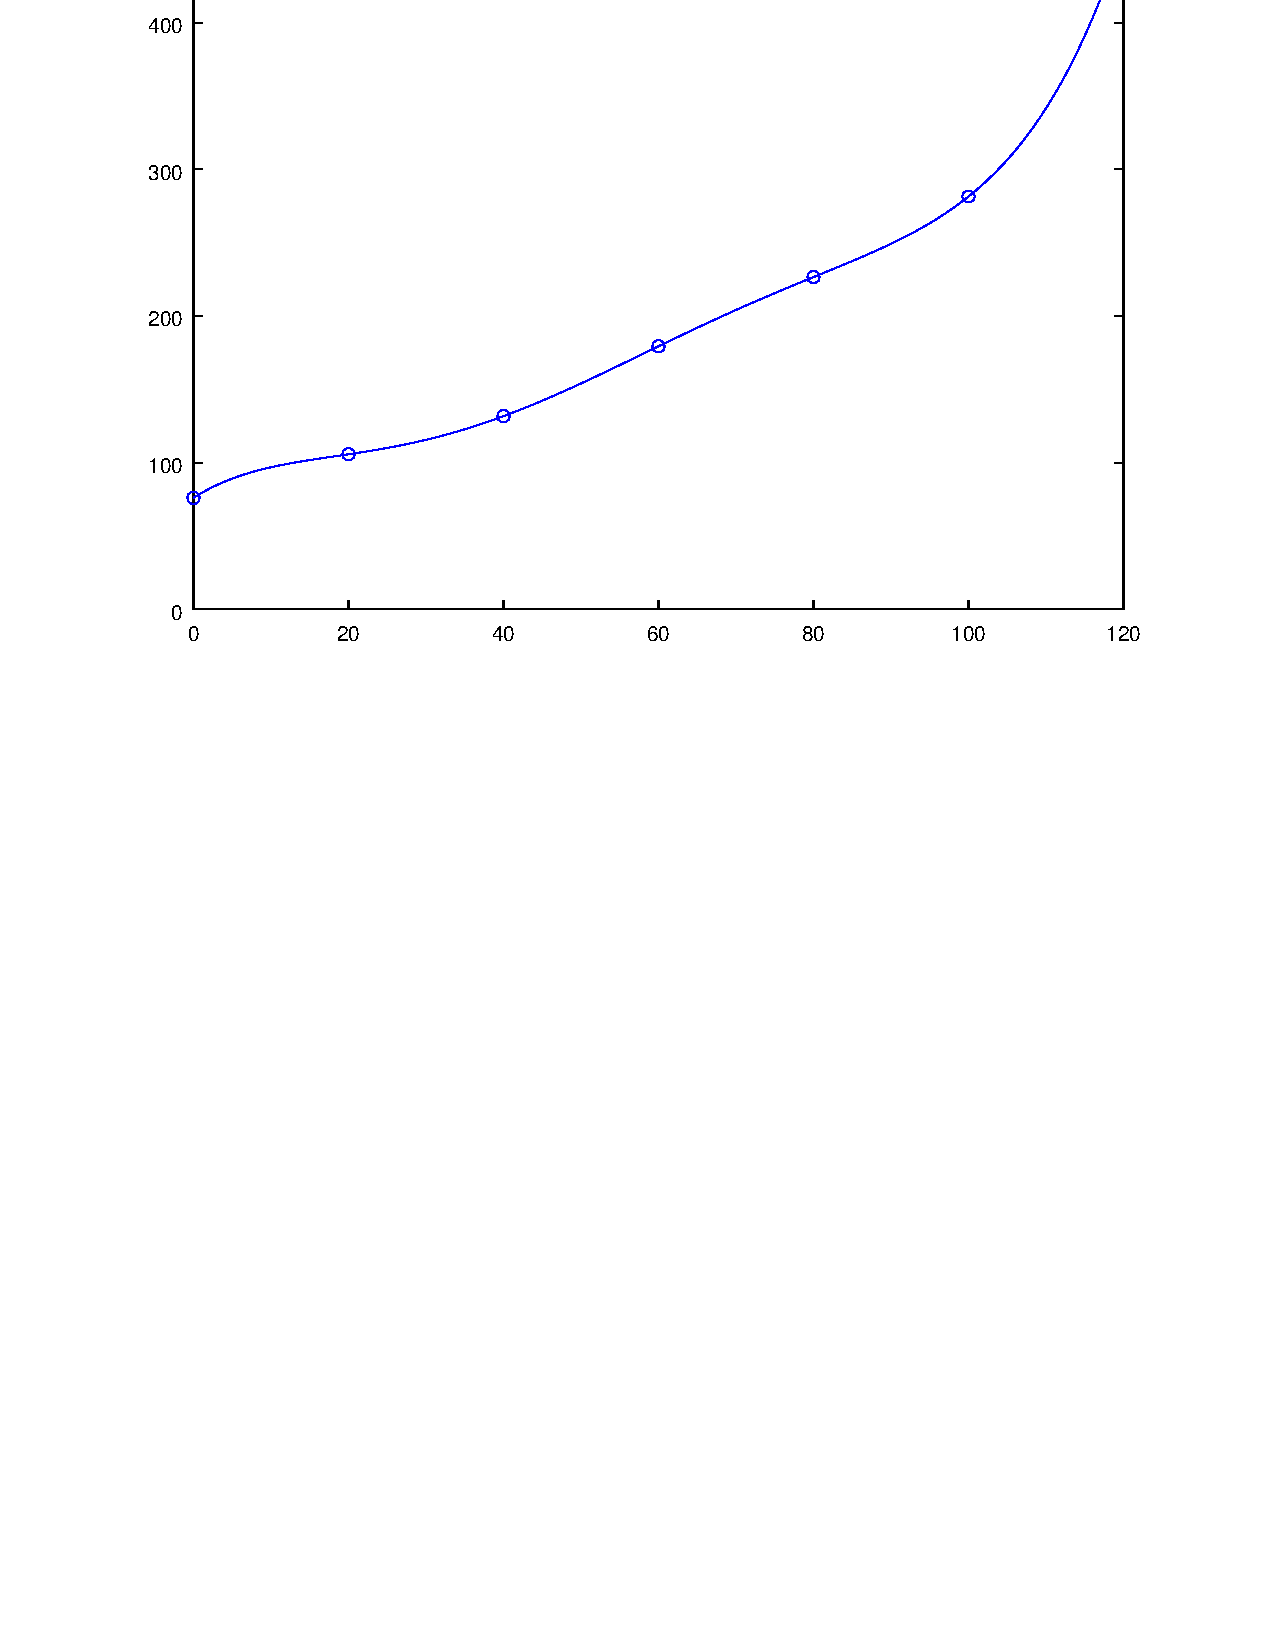
\includegraphics[scale=.5]{../octave/p1.pdf}
\item
the newton form constants are independent of the number of additional points, so the zero order constant is the first constant of the first order and the first constant of the second order.  Thus I can simply give the second order constants and the first two are the first order constants and the first one is the zero order constant.
\lstinputlisting{../octave/q81b.m}
\lstinputlisting{../octave/d6.txt}
Noting that the sum of the absolute error is extremely small, order $10^{-9}$, for $20000$ points we can say that the two are identical, within machine error.
\end{enumerate}
\begin{exercise}

8.2
\end{exercise}
The Lagrange form of the third order polynomial would be 
$$P(x)=\sum_{i=k-3}^{k}f(i)*\prod_{j\in[k-3,k]:j\neq i}\frac{x-x_j}{x_i-x_j}$$
\lstinputlisting{../octave/d7.txt}
since $1.21525$ is closer to $2$, it is our next $x$ value.
\begin{exercise}

8.7
\end{exercise}
\lstinputlisting{../octave/q87.m}
\lstinputlisting{../octave/herm.m}
I will present my results as a graph, however the results for the Hermite polynomial are so close that one would need a zoom to make out the difference.  Thus I also give a difference plot between the Hermite polynomial and the function.\\
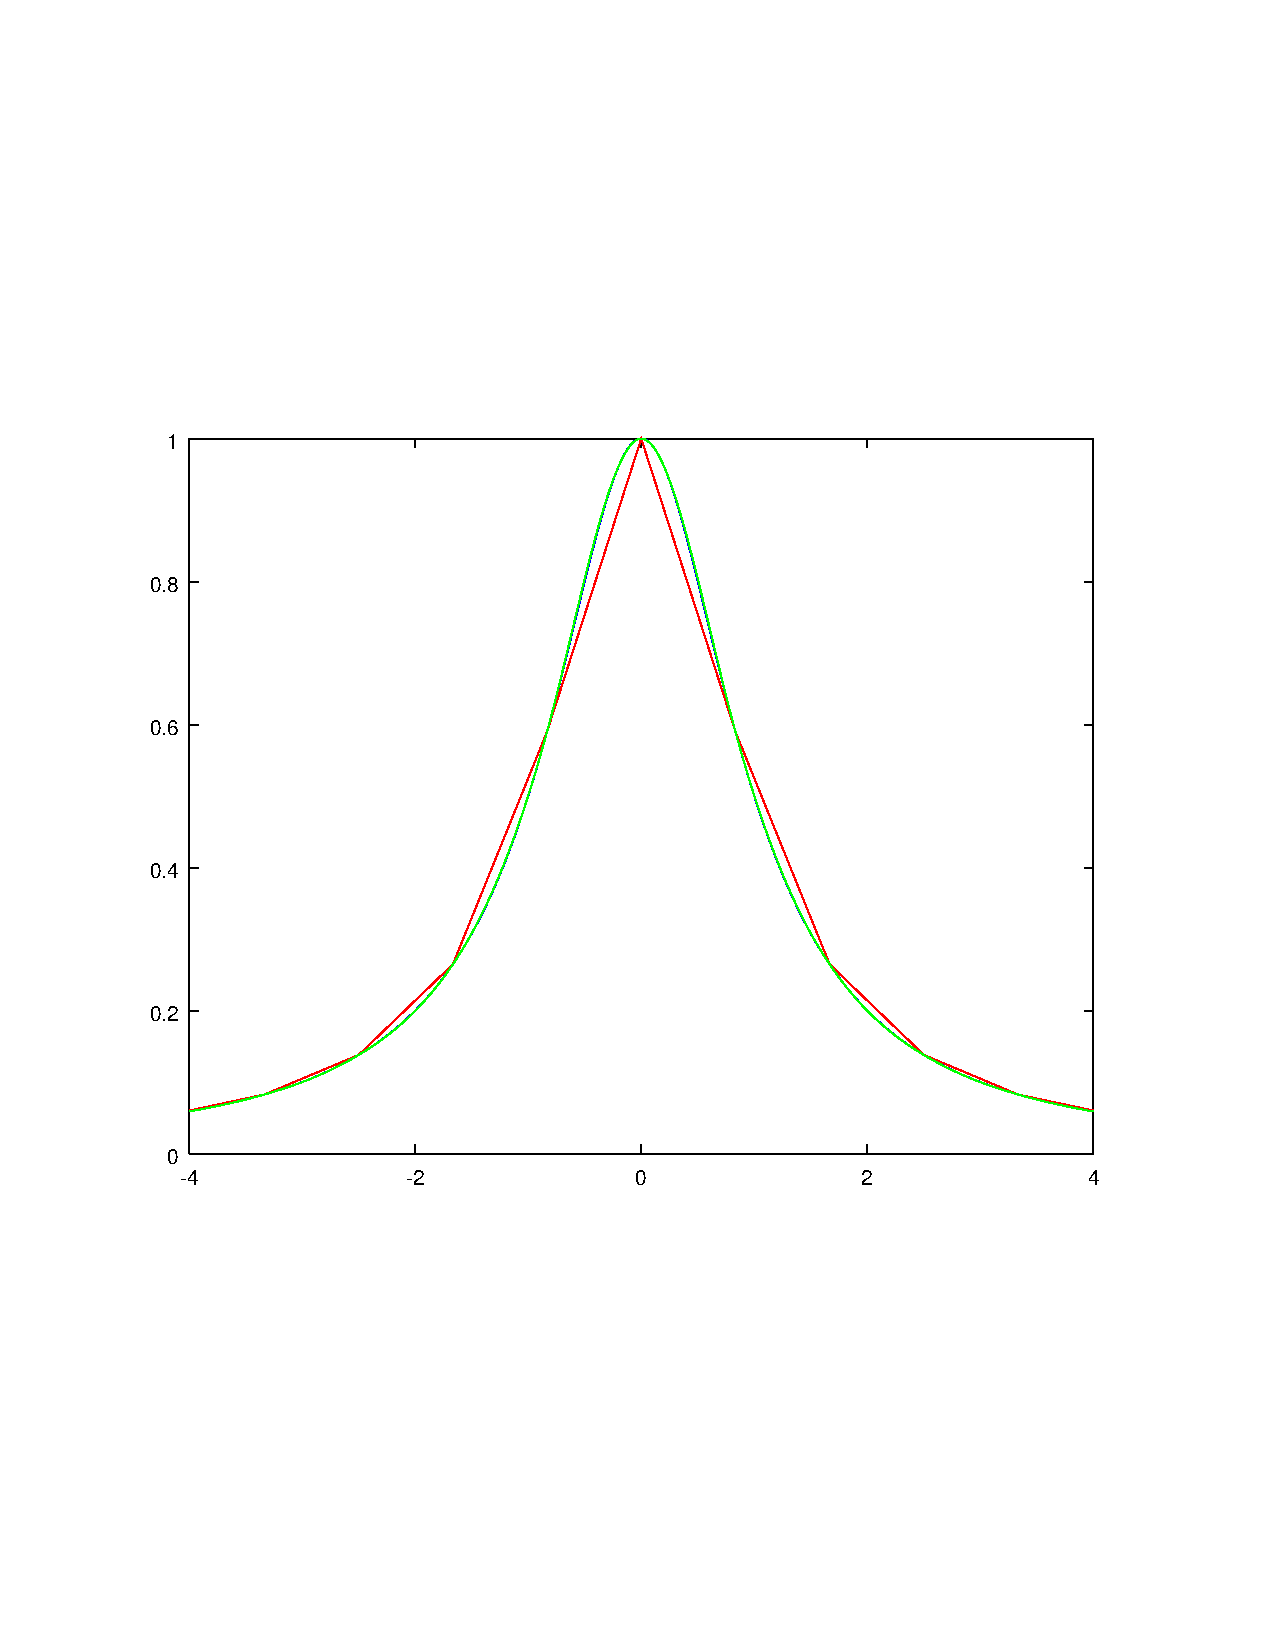
\includegraphics[scale=.7]{../octave/herm.pdf}\\
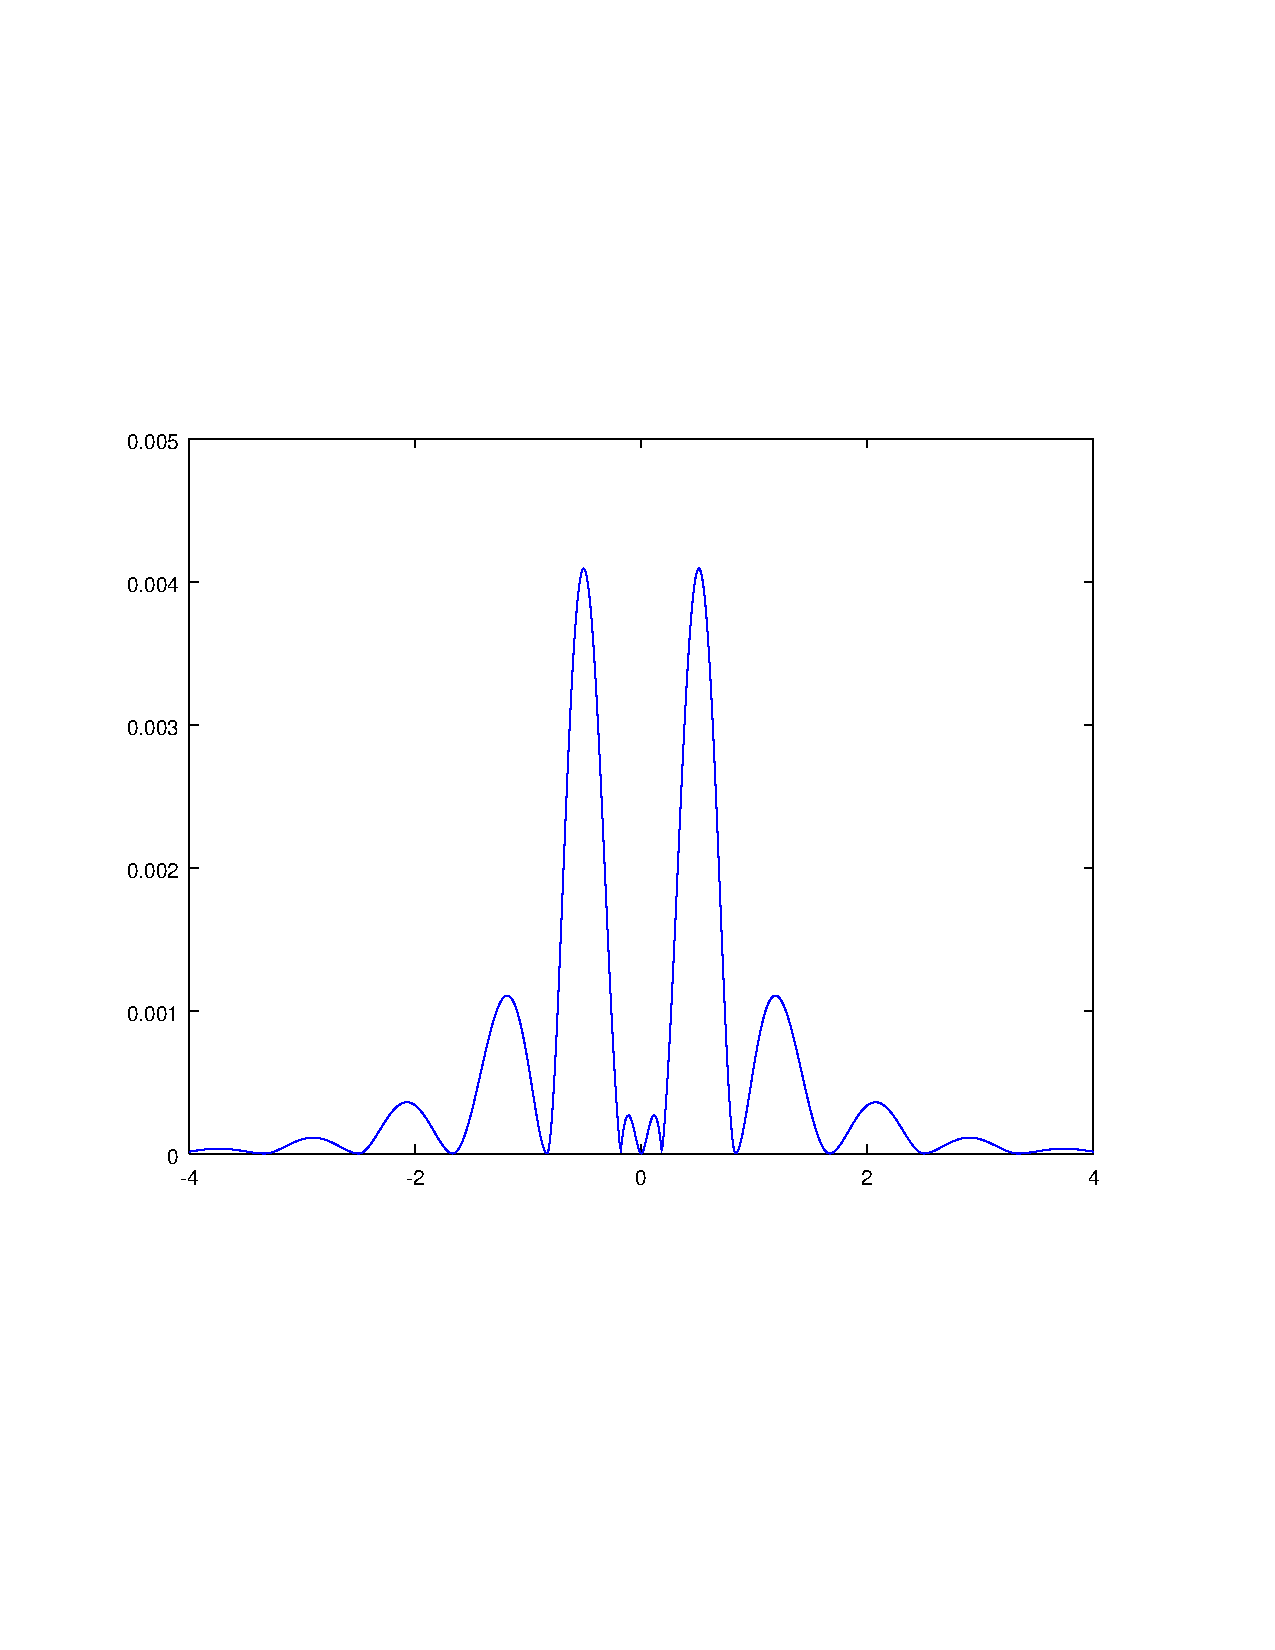
\includegraphics[scale=.7]{../octave/herm2.pdf}
\begin{exercise}

8.8
\end{exercise}
\lstinputlisting{../octave/q88.m}
\lstinputlisting{../octave/rest.m}
\lstinputlisting{../octave/d8.txt}
\begin{exercise}

7.14
\end{exercise}
\lstinputlisting{../octave/q714.m}
\lstinputlisting{../octave/d9.txt}
The errors for the low order constants have more error then the high order ones.
\end{document}